\documentclass{article}
\usepackage{listings}
\usepackage{graphicx}
\usepackage{amsmath}
\usepackage{minted}
\usepackage[margin=1in]{geometry}
\usepackage{xcolor}


\definecolor{codegreen}{rgb}{0,0.6,0}
\definecolor{codegray}{rgb}{0.5,0.5,0.5}
\definecolor{codepurple}{rgb}{0.58,0,0.82}
\definecolor{backcolour}{rgb}{0.95,0.95,0.99}
\lstdefinestyle{mystyle}{
    backgroundcolor=\color{backcolour},   
    commentstyle=\color{codegreen},
    keywordstyle=\color{magenta},
    numberstyle=\tiny\color{codegray},
    stringstyle=\color{codepurple},
    basicstyle=\ttfamily\footnotesize,
    breakatwhitespace=false,         
    breaklines=true,                 
    captionpos=b,                    
    keepspaces=true,                 
    numbers=left,                    
    numbersep=5pt,                  
    showspaces=false,                
    showstringspaces=false,
    showtabs=false,                  
    tabsize=2
}
\lstset{style=mystyle}

\begin{document}
\title{ELCT 432: Computer Assignment \#4, Lossless Data Transmission}
\author{Jacob C. Vaught}
\date{September 24th, 2023}
\maketitle
\section*{Transmitter[40 Points]}
\subsubsection*{IQ Data Preparation and Transmission}
The IQ data is prepared from the grayscale image. The carrier frequency and sample frequency are set, and the IQ data is normalized.

\subsubsection*{Signal Analysis}
The code uses the `analyzeIQdata` function to plot various features of the signal like time-domain, IQ data, PSD, and IQ diagram.

\subsubsection*{SDR Transmission and Reception}
The code uses SDRs to transmit and receive the IQ data, followed by a series of synchronization and correction steps.

\subsubsection*{MATLAB Code}
\lstinputlisting[language=Octave]{transmitter_Basic.m}
\newpage
\subsection*{Analysis and Discussion}
\subsubsection*{Time-domain, IQ data, and PSD}
Every part of the signal is in-Phase. The signal features a sync function that linearly ascends from an amplitude of 0 to 1 over a 5 ms time span (had to adjust this to 10 ms after consulting the instructions). The additional 12 ms is allocated for transmitting the signal using a carrier wave. As for the Power Spectral Density (PSD), it exhibits a primary peak at 910 MHz and gradually tapers off into adjacent frequencies. The data's upper limit is fixed at 0.8 and the lower limit at 0, in compliance with the guidelines (I must confess that I overlooked this detail initially, which led me to make revisions later on).
\begin{center}
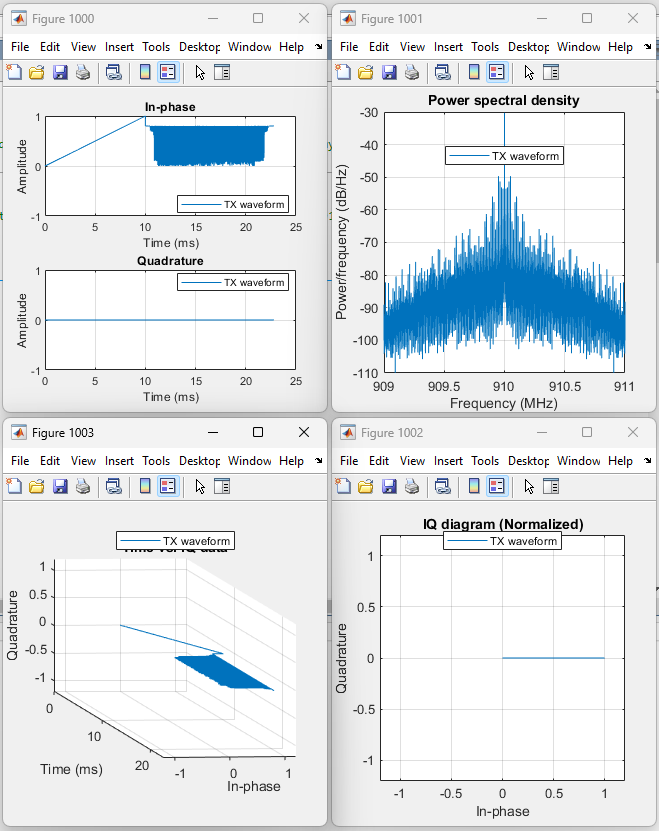
\includegraphics[scale=0.85]{Transmit_Basic.png}
\end{center}


\subsubsection*{Comparison to Conventional AM}
The signal exhibits characteristics akin to Amplitude Modulation (AM) in that it uses an 8-bit value to modulate the amplitude of the carrier frequency. This results in the signal bandwidth varying dynamically in accordance with the message. Similar techniques leveraging amplitude modulation exist, often utilizing a binary scheme. In such configurations, only two states—high or low—are possible. This binary approach enhances the system's reliability, particularly in noisy environments.


\section*{Channel[10 Points]}
\begin{center}
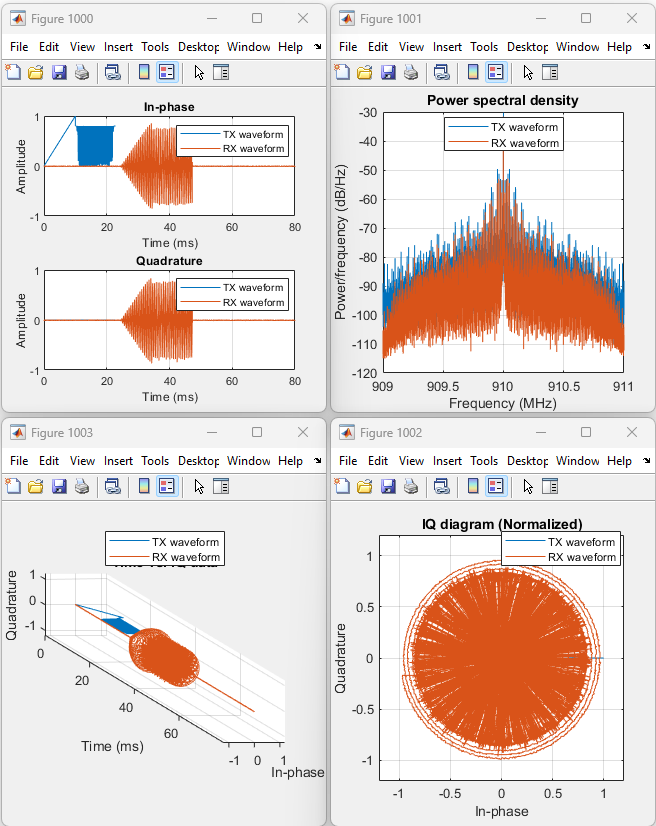
\includegraphics[scale=0.85]{Channel.png}
\end{center}
\subsubsection*{Discussion}
The received signal possesses both quadrature and in-phase components, although the original signal was purely in-phase. This discrepancy is likely attributable to physical limitations and inaccuracies inherent in the actual hardware. Additionally, a phase shift is observed in the signal, which presents an opportunity for further signal correction.

The Power Spectral Density (PSD) plot reveals that the actual power of the received signal is marginally lower than what was initially transmitted. Such a phenomenon is typical in wireless communication systems and is an expected characteristic when using antennas.

\section*{Receiver[50 Points]}
\subsubsection*{Results}
Transmitted Figure:
\begin{center}
\newline

\includegraphics[scale=0.3]{TX.png}
\end{center}
\newline
Received Figure:
\begin{center}
\newline
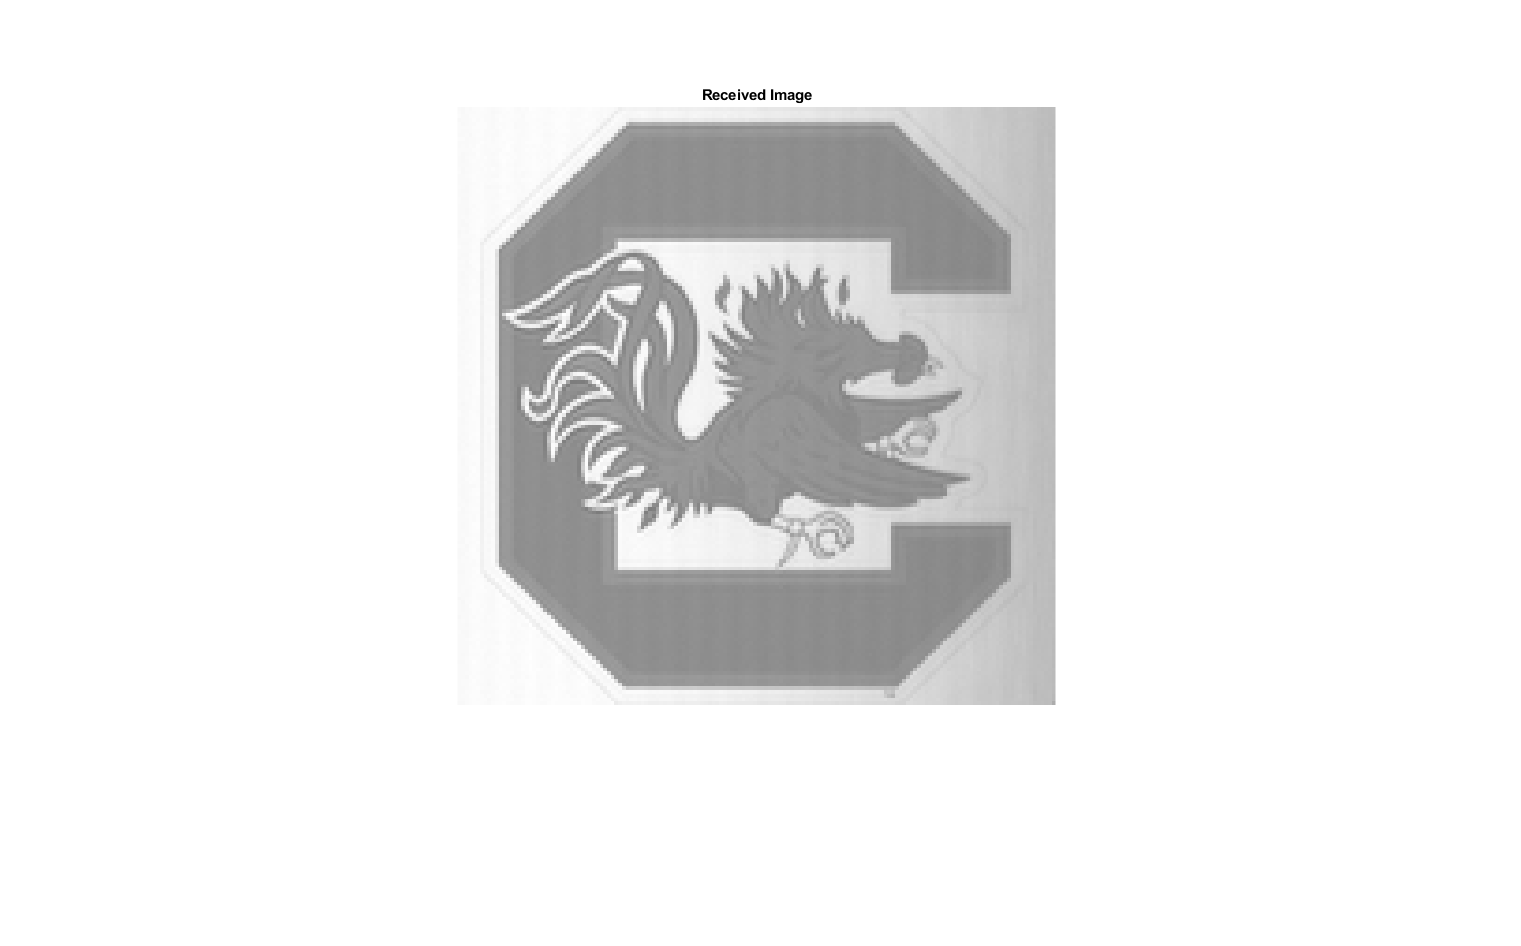
\includegraphics[scale=0.3]{RX.png}
\end{center}
\newpage
IQ vs. Time Figure:
\begin{center}
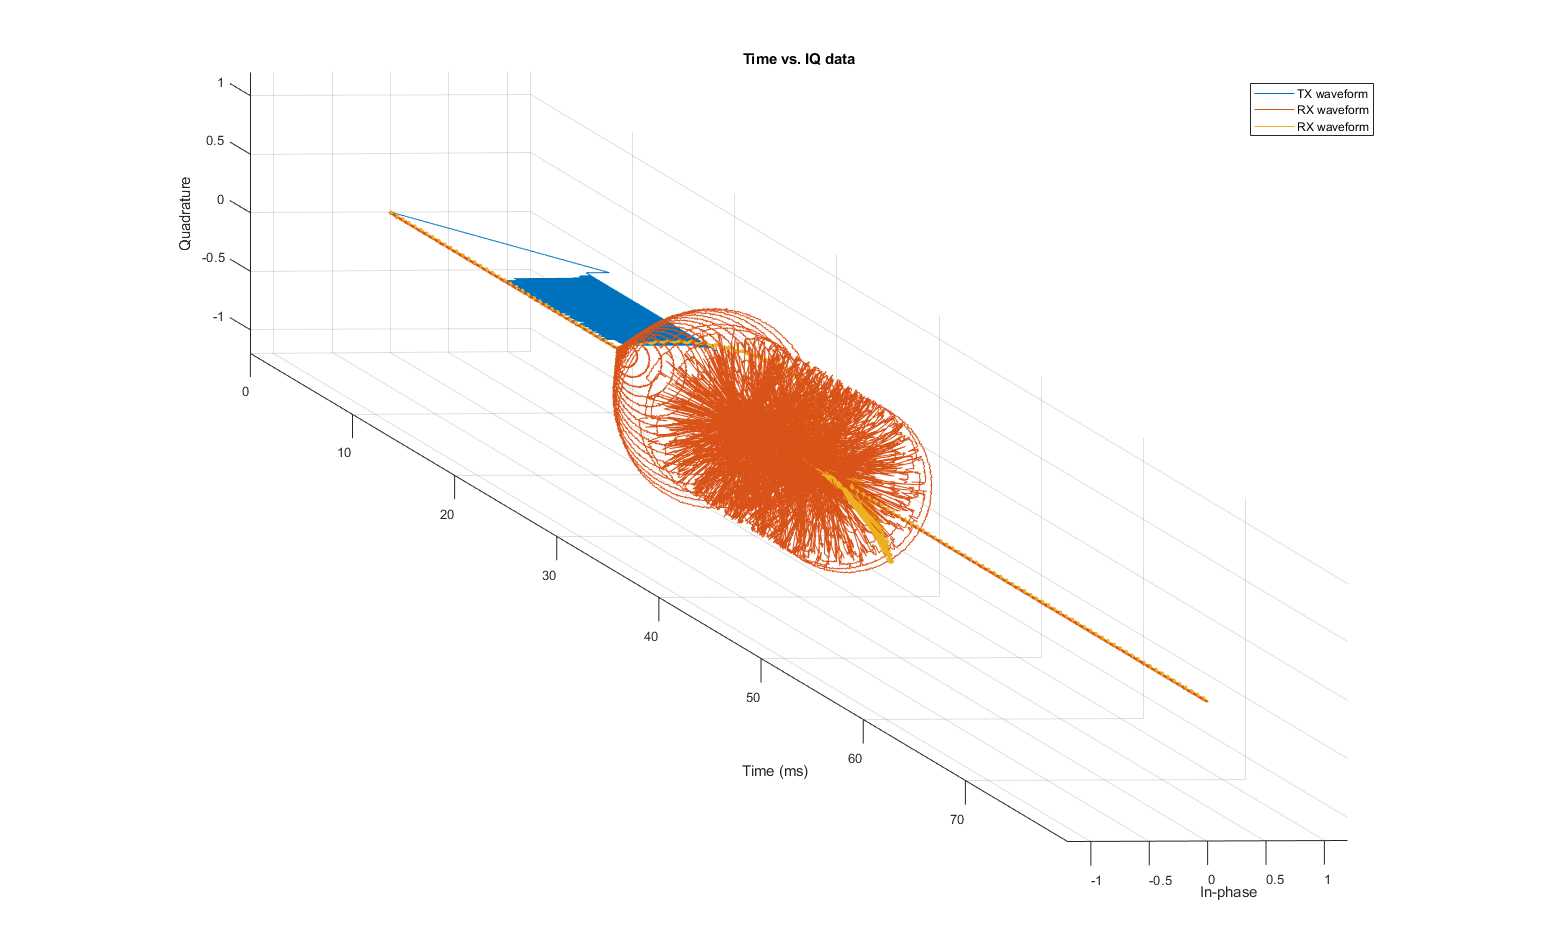
\includegraphics[scale=0.4]{TIQ.png}
\end{center}
\newline
Normalized IQ Figure:
\begin{center}
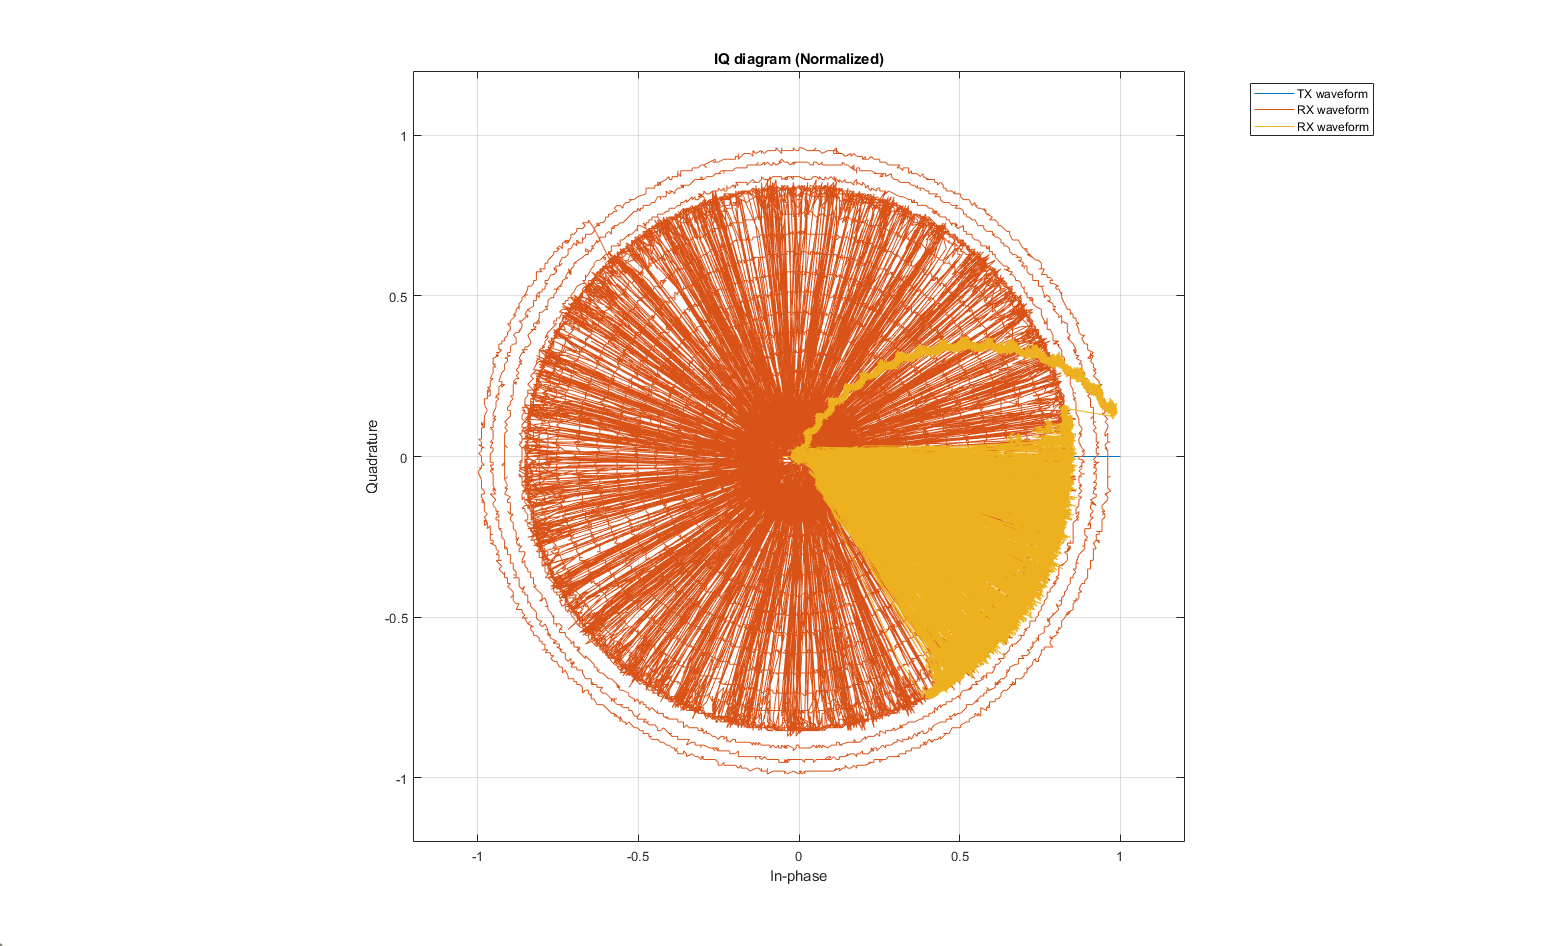
\includegraphics[scale=0.4]{IQN.png}
\end{center}
\newpage
Power Spectral Density Figure:
\begin{center}
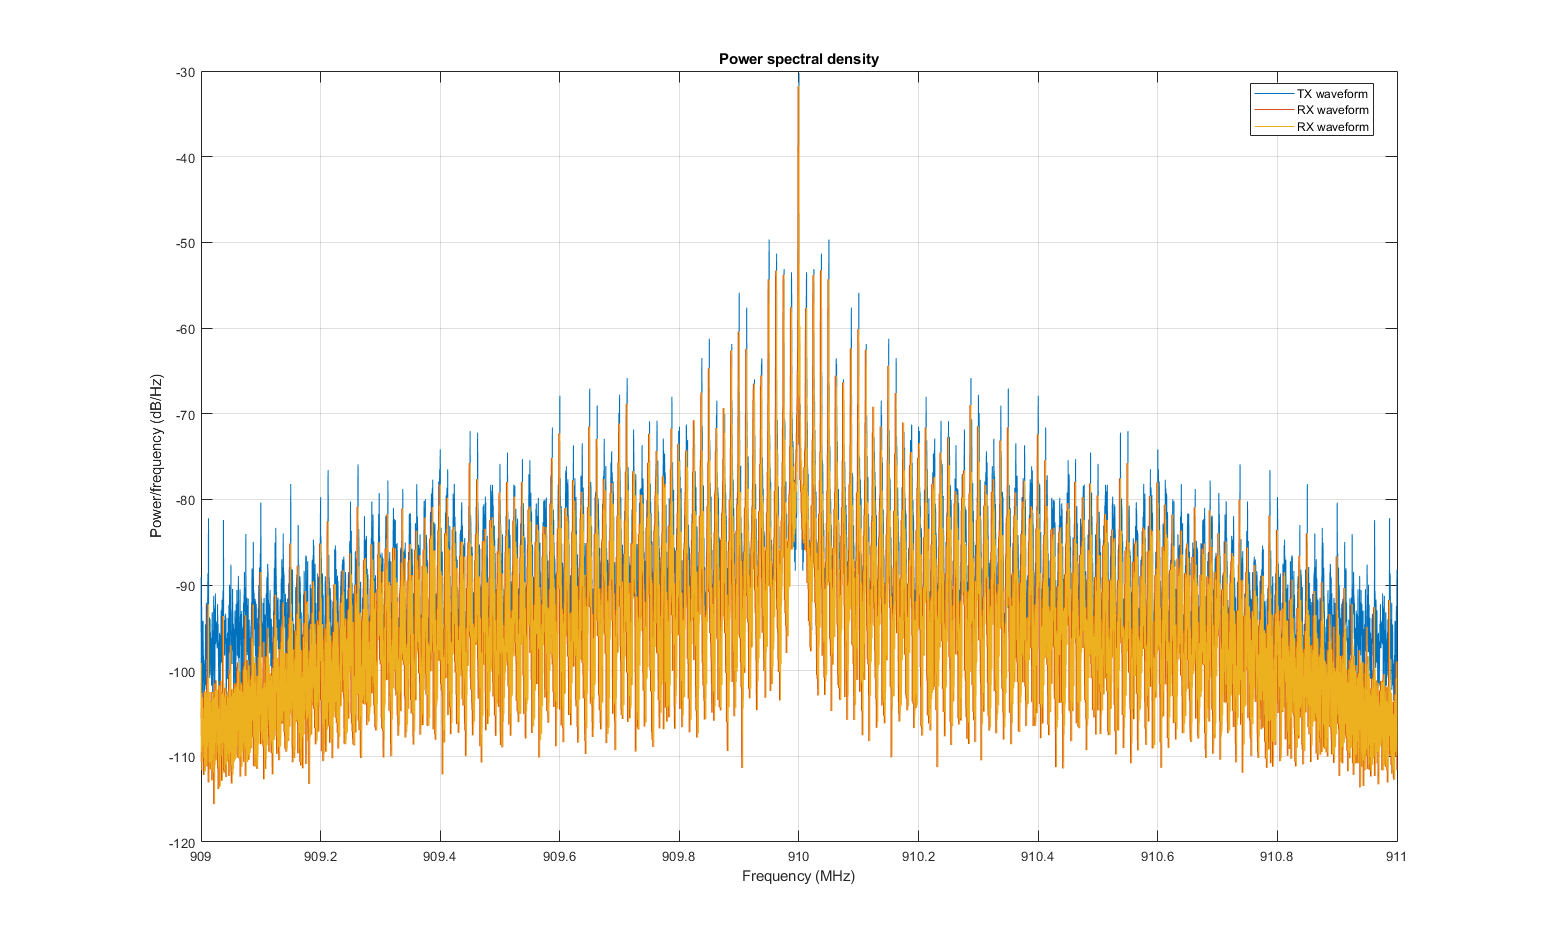
\includegraphics[scale=0.4]{PSD.png}
\end{center}
\subsection*{Code Overview}
The code mainly includes five significant steps:

\begin{itemize}
    \item Coarse Synchronization
    \item CFO Estimation
    \item CFO and Phase Correction
    \item Fine Time Synchronization using Maximum Likelihood Estimation
    \item Displaying the Received Image
\end{itemize}

\subsubsection*{Saving Variables}
The function \texttt{save('Received\_Data.mat', 'fc', 'fsample', 'IQdataRX', 'options');} is used to save variables to a \texttt{.mat} file for later analysis(This is primarily a test function for interesting edge cases).

\subsubsection*{Step 1a: Coarse Sync}
\textbf{How:} 
The coarse synchronization is carried out using the \texttt{max} function, which is applied to the real part of the received IQ data. The maximum point's index is used to calculate the corresponding coarse time by dividing it by the sampling frequency.
\newline \textbf{Why:} 
Coarse synchronization serves as the initial alignment of the receiver with the incoming data. It acts as a fundamental reference point, narrowing down the area where subsequent, more accurate synchronization methods will work. This step is crucial for the efficiency and accuracy of the entire system.

\subsubsection*{Helper Function: calcCoarseTime}
\textbf{How:}
The \texttt{calcCoarseTime} function calculates the coarse time by dividing the maximum point's index (\texttt{nCoarseSync}) by the sampling frequency (\texttt{fsample}).
\newline \textbf{Why:}
Converting this index into a time measure is crucial as it sets a time-based frame of reference for all the subsequent steps, making the signal processing more interpretable and aligned with real-world timing.

\subsubsection*{Step 2: CFO Estimation}
\textbf{How:}
A segment of IQ data is extracted around the coarse synchronization point, and its Fast Fourier Transform (FFT) is computed. The frequency that has the maximum magnitude in this transformed data is used as the CFO estimate.
\newline \textbf{Why:}
CFO, if uncorrected, can significantly impair the demodulation process, causing a degradation in data integrity. Thus, estimating and correcting it is pivotal for maintaining the system's performance.

\subsubsection*{Helper Function: performFFT}
\textbf{How:}
The \texttt{performFFT} function takes the segment of the IQ data and performs FFT, following it up with an FFT shift to center the zero frequency.
\newline\newline \textbf{Why:}
FFT is a computationally efficient method for converting the time domain signal into frequency domain, making it much easier to identify CFO. The FFT shift is a standard practice to simplify the analysis of the transformed data.

\subsubsection*{Step 3: CFO and Phase Correction}
\textbf{How:}
After estimating the CFO, it is corrected using a complex exponential function applied to the IQ data. Phase error is then estimated and corrected.
\newline \textbf{Why:}
CFO and phase corrections are essential for ensuring that the demodulation process correctly interprets the received data. Without these corrections, data integrity could be compromised.

\subsubsection*{Step 4: Fine Time Sync using Maximum Likelihood Estimation}
\textbf{How:}
A range is defined around the coarse sync point, and the maximum value of the derivative of the real part of the signal within this range is identified. This point serves as the fine synchronization index.
\newline \textbf{Why:}
Fine synchronization refines the initial alignment, significantly enhancing the subsequent data decoding's accuracy. Maximum Likelihood Estimation is often used for its robustness and accuracy in finding this point.

\subsubsection*{Step 5: Display Image}
\textbf{How:}
The received image is displayed by extracting the relevant portion of the IQ data, scaling it, and then reshaping it into an image.
\newline \textbf{Why:}
This step serves as a practical validation of all the previous steps and provides a user-friendly representation of the received data. Successful image display confirms the system's effectiveness.

\subsubsection*{Helper Function: displayReceivedImage}
\textbf{How:}
This function takes the IQ data, scales it, and reshapes it to produce a 160x160 image, which is then displayed.
\newpage
\subsection*{Discussion on CFO: Is it needed?}
In the context of our wireless communication system, CFO correction is indispensable for several compelling reasons:

\begin{enumerate}
    \item \textbf{Data Integrity}: The presence of CFO can introduce phase rotations in the received IQ data, thereby increasing the likelihood of symbol errors during the demodulation process. Given the high data rates[2MHz] and low error tolerance in our system, ensuring data integrity is paramount.
    
    \item \textbf{Spectral Efficiency}: CFO has the potential to spread the signal's spectrum, leading to adjacent channel interference. Our system is designed for environments with tight spectral constraints[10 MHz?], making CFO correction essential for optimal operation.
    
    \item \textbf{Real-world Conditions}: Due to hardware imperfections and environmental influences, perfect synchronization between the transmitter and receiver is practically impossible, rendering CFO almost inevitable.
\end{enumerate}

Thus, given the specific requirements and constraints of our application, CFO correction is not just advisable but essential for maintaining high system performance and data integrity.
\subsection*{MATLAB Code}
\lstinputlisting[language=Octave]{receiver.m}
\newpage
\section*{Exploration of Alternative Image Transmission Strategies}

In tackling the problem at hand, I engineered multiple alternative programs aimed at facilitating image transmission. Each of these distinct approaches carried unique advantages and limitations, influencing the efficiency, robustness, and fidelity of the transmitted images.
Additionally, my methods utilize a different scale factor and sync function than the assignment had provided initially. 

\subsection*{Binary Black and White System}

The first foray into alternative methodologies was an elementary binary system solely committed to black and white pixels. In this model, each pixel could only assume one of two states, black or white, obviating the need for any grayscale representation. Consequently, the output signal's amplitude was either zero or scaled to unity. This simplicity conferred unparalleled robustness to the signal, albeit at the expense of photo quality.

\subsection*{Three-Bit Color System}

My second approach embraced color by allocating a single bit to represent each pixel's hue. This modest bit-depth still enabled the transmission of colored images, again relying on a binary signaling format. The trade-off here was between chromatic richness and transmission simplicity.

\subsection*{Three-Bit Grayscale System}

The third approach delved into grayscale imagery but with a confined bit-depth of 3 bits per pixel. This limited palette afforded eight different shades of gray, striking a middle ground between the binary black and white system and more nuanced grayscale methods.

\subsection*{Eight-Bit Grayscale System}

Transitioning to a more sophisticated scheme, the fourth methodology exploited an 8-bit grayscale system. This configuration could manifest the full spectrum of 255 shades of gray, offering superior image fidelity while still adhering to a binary signaling format.

\subsection*{Nine-Bit Full-Color System}

Finally, the most intricate scheme deployed a 3-bit allocation for each primary color (Red, Green, Blue), resulting in a 9-bit representation per pixel. Though computationally demanding, this approach rendered the most vibrant and realistic images.

\subsection*{Unimplemented Features}

Among the features I had on my roadmap but couldn't execute were compression and error-correction algorithms. These additional layers could have further narrowed the performance gap between my "digital" approaches and the original "analog" design, particularly considering the latter's 255-value data point granularity.

\subsection*{Advantages of My Approaches}

The paramount advantage of my alternative transmission methods was their resilience to both noise and CFO (Carrier Frequency Offset). Unlike the original system, my strategies mostly operated on the absolute values of the signal, substantially mitigating the need for phase correction or CFO adjustments. This inherent robustness led to more consistent and reliable performance, even under suboptimal tuning conditions.

\subsection*{An Important Observation for the Reader}

As you peruse the subsequent material, one notable aspect emerges: the majority of these alternative transmission techniques exhibit minimal reliance on precise Carrier Frequency Offset (CFO) adjustments. This phenomenon is vividly illustrated by the sinusoidal artifacts present in the IQ phase diagrams corresponding to each method. The primary reason for this inherent robustness lies in the utilization of binary transmission schemes.

While these binary methods offer excellent tolerance to inaccuracies in CFO, their robustness comes at a cost. Specifically, for applications requiring high data transmission rates or over extended durations, relying solely on binary schemes would become increasingly impractical. Augmenting the existing approaches with frequency modulation, phase modulation, or even multi-level binary transmission—such as quaternary signaling that allows four distinct signal points—would significantly improve data throughput. In this manner, you can double the number of bits transmitted per unit time while potentially enhancing the system's overall efficiency and reliability. Naturally, increasing the number of bits transmitted per period—while maintaining the same carrier frequency—leads to a rise in the error rate. This necessitates the implementation of more robust error correction techniques, which in turn further elevate the computational overhead.


\section*{Results}
\subsection*{3 Bit BW image}
\begin{center}
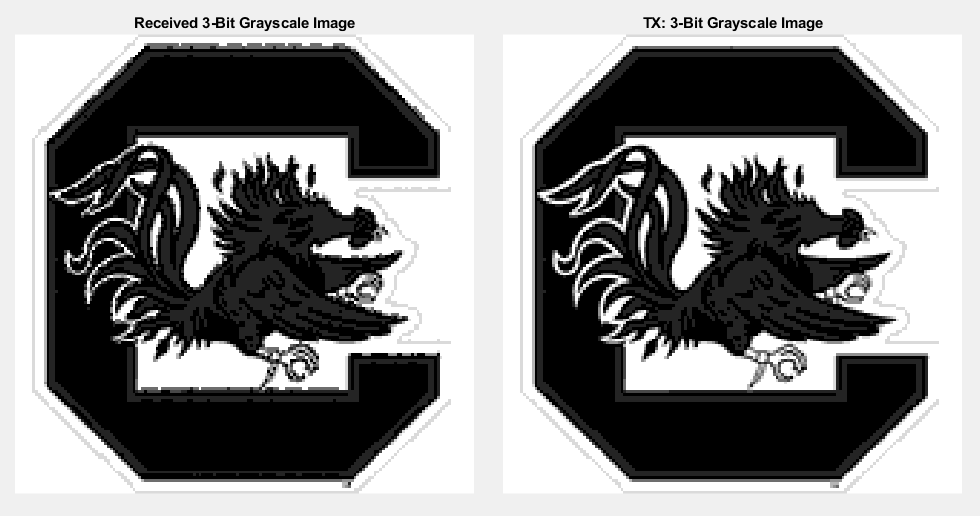
\includegraphics[scale=0.6]{3BW_image.png}
\end{center}
\begin{center}
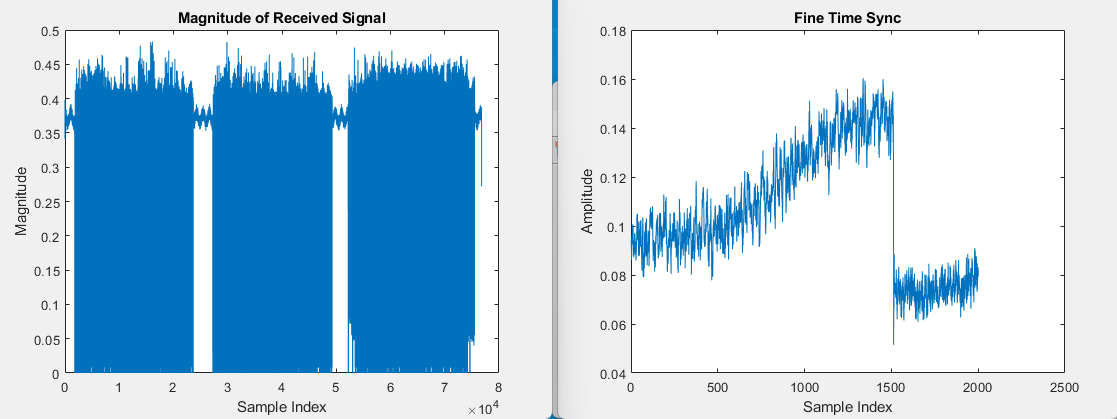
\includegraphics[scale=0.5]{3BW_Sync.png}
\end{center}
\begin{center}
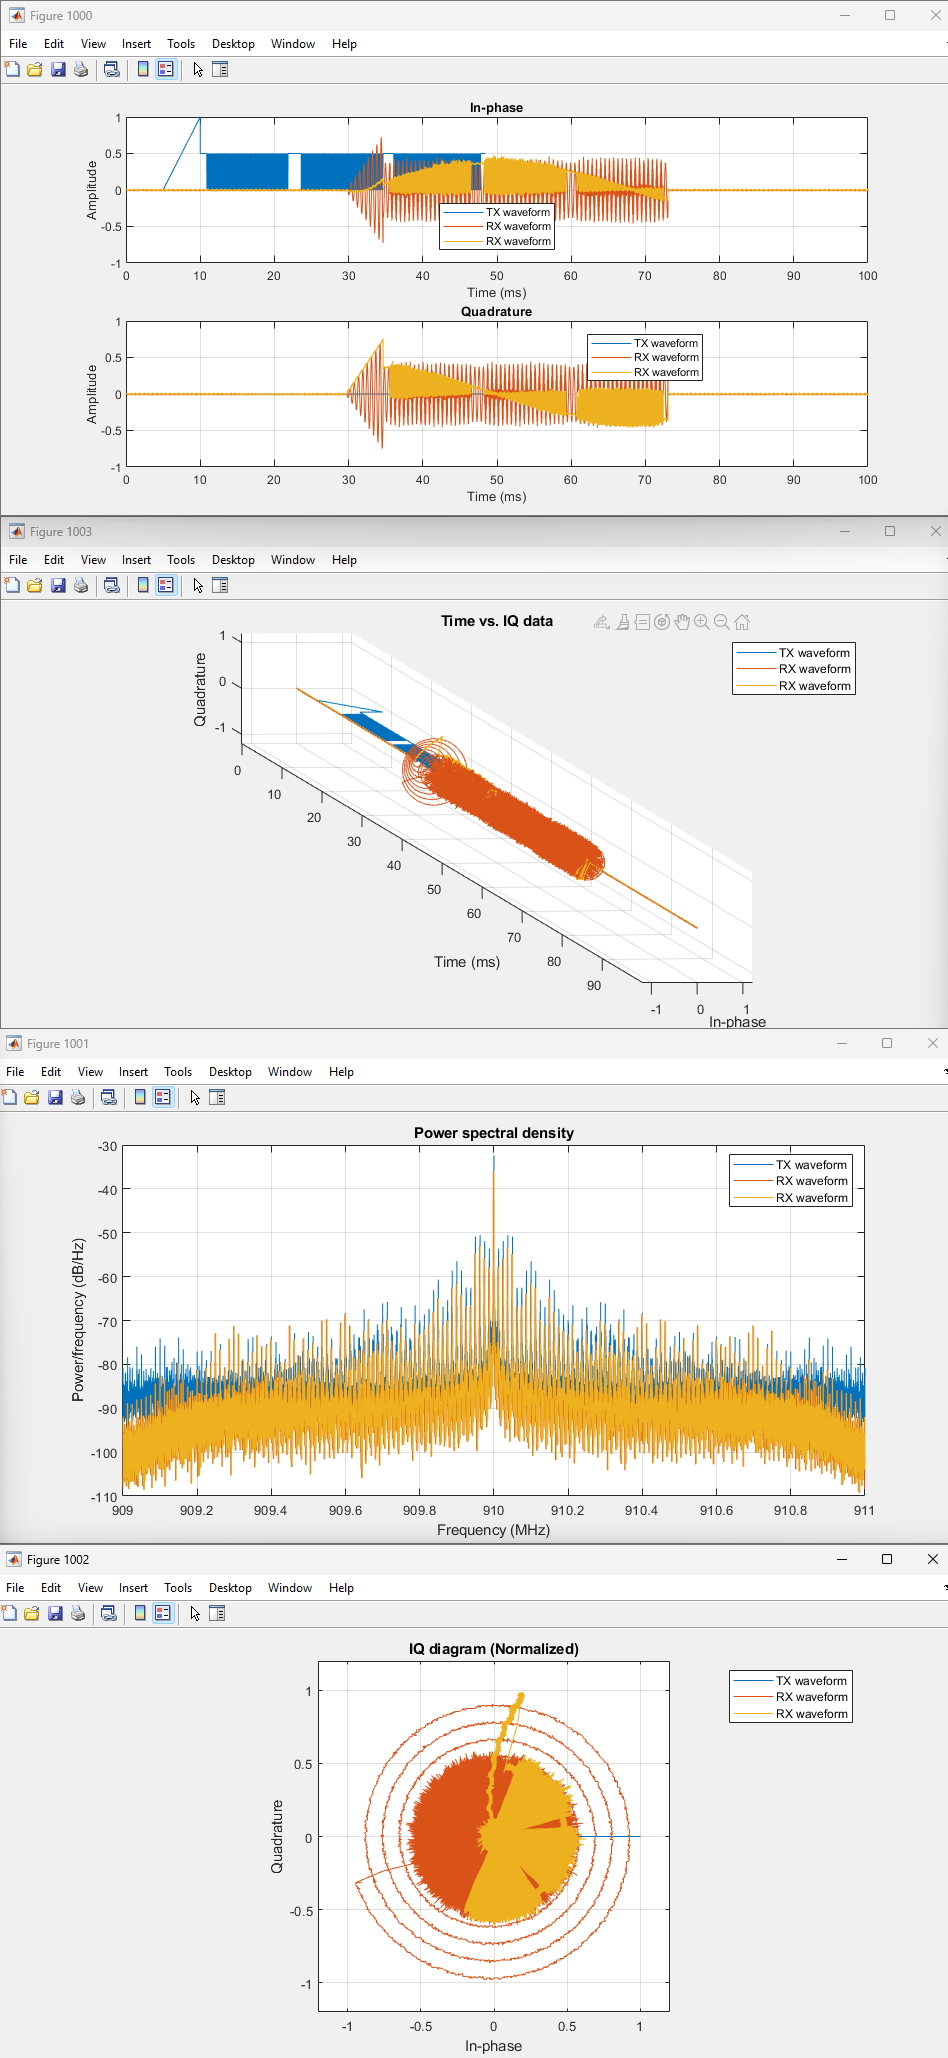
\includegraphics[scale=0.42]{3BW_results.png}
\end{center}


\newpage
\subsection*{1 Bit Color image}
\begin{center}

\includegraphics[scale=0.6]{1C_image.png}
\end{center}
\begin{center}
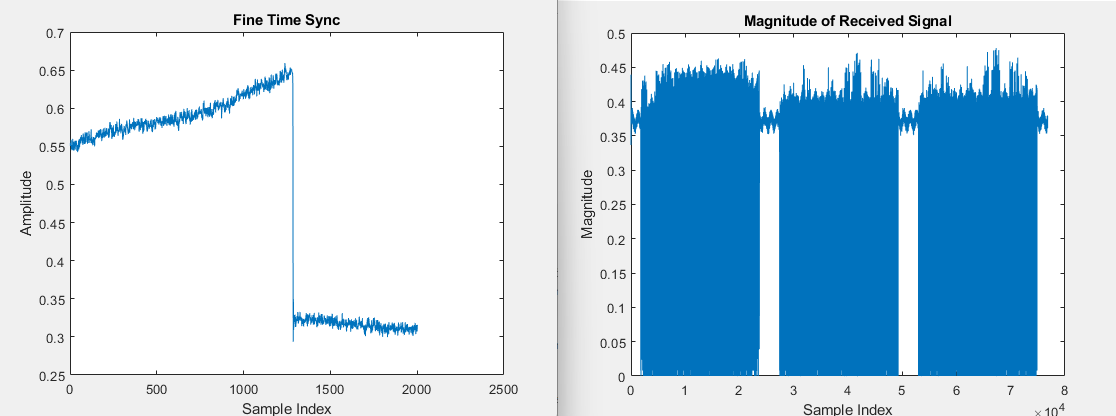
\includegraphics[scale=0.5]{1C_Sync.png}
\end{center}
\begin{center}
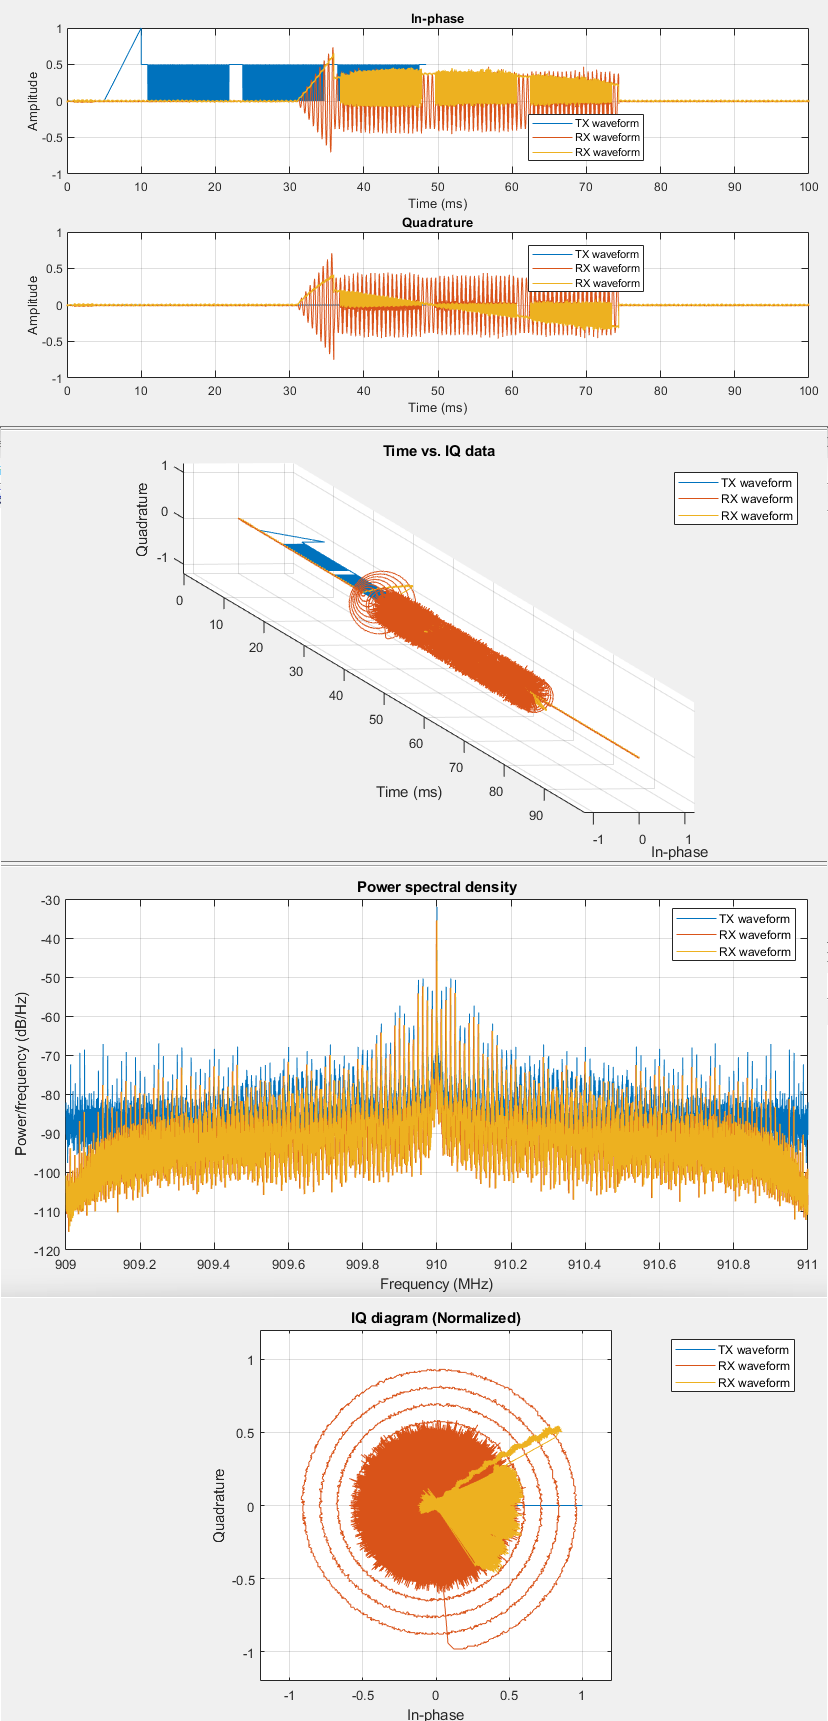
\includegraphics[scale=0.42]{1C_results.png}
\end{center}

\newpage
\subsection*{3 Bit Color image}
\begin{center}
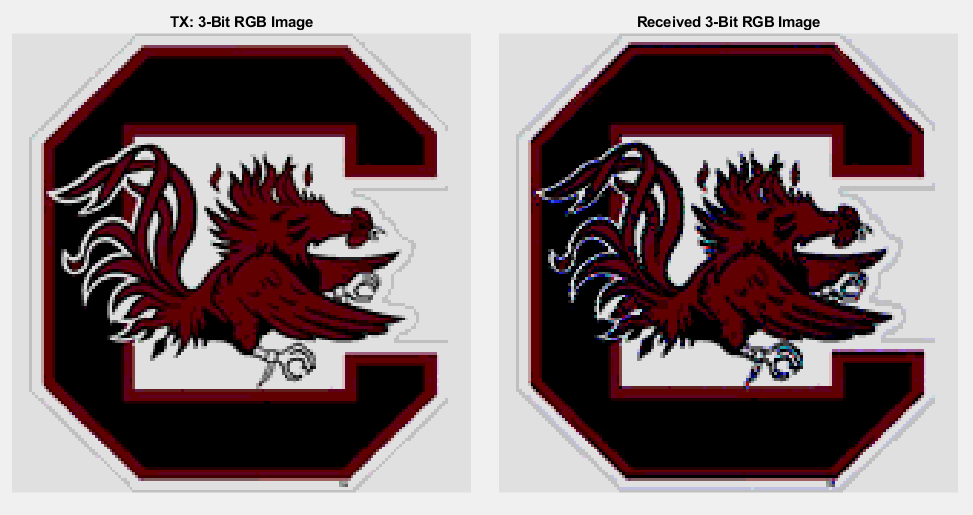
\includegraphics[scale=0.6]{3C_image.png}
\end{center}
\begin{center}
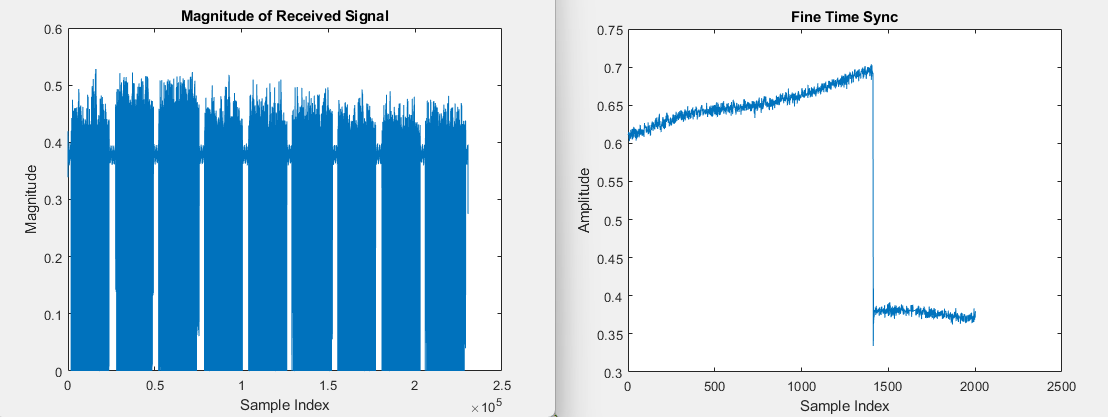
\includegraphics[scale=0.5]{3C_Sync.png}
\end{center}
\begin{center}
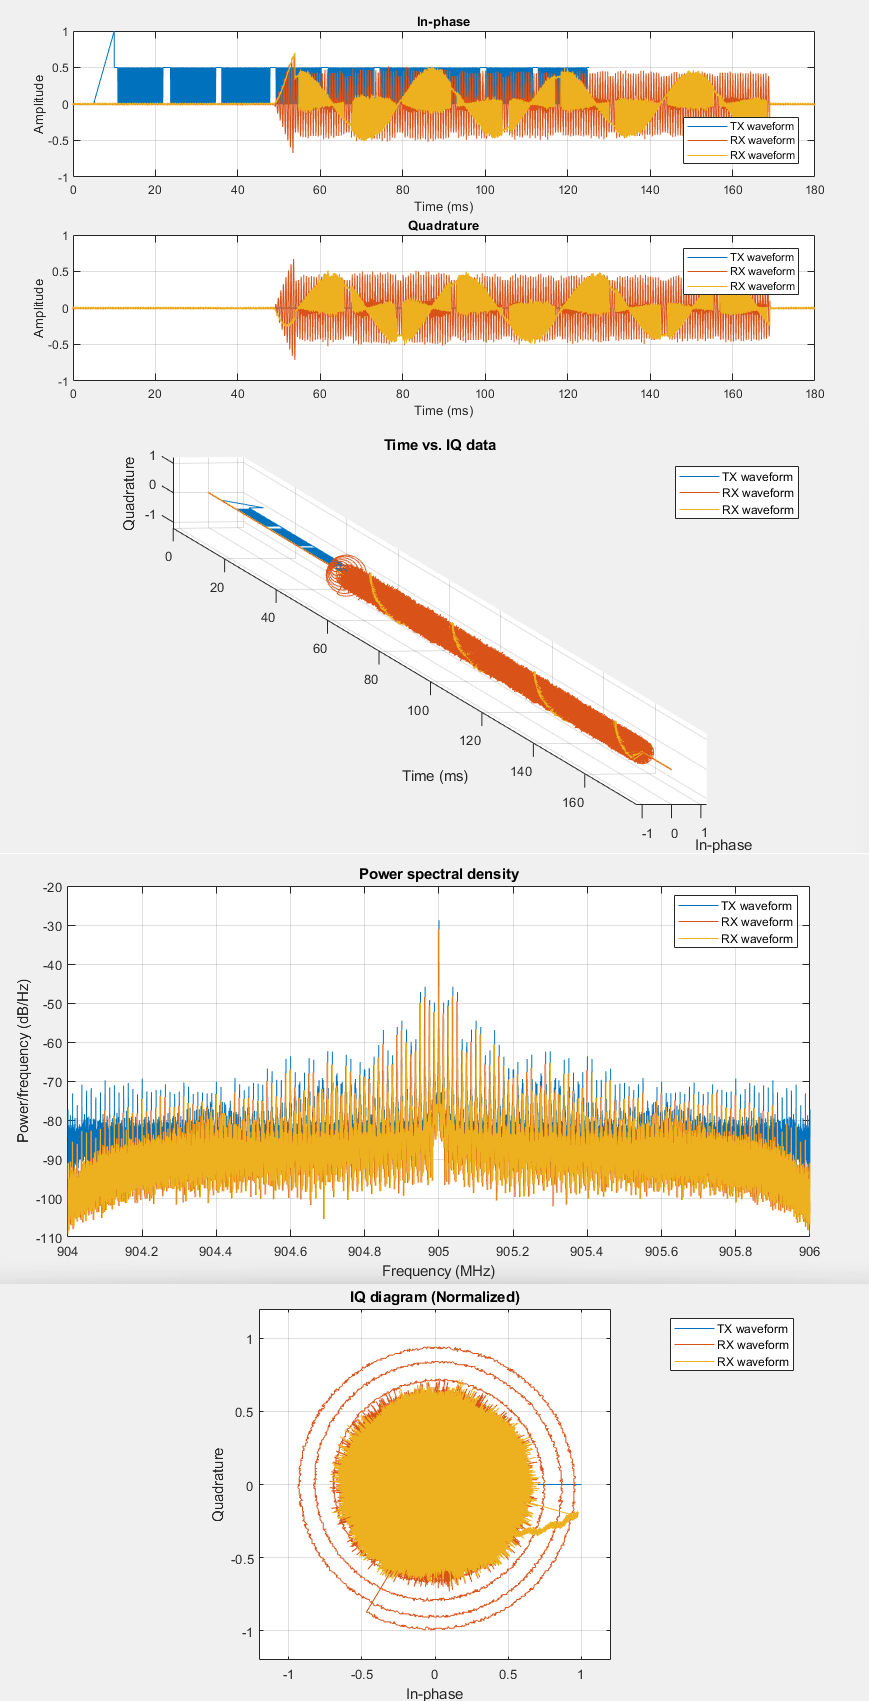
\includegraphics[scale=0.42]{3C_results.png}
\end{center}

\newpage
\subsection*{8 Bit Grayscale image}
\begin{center}
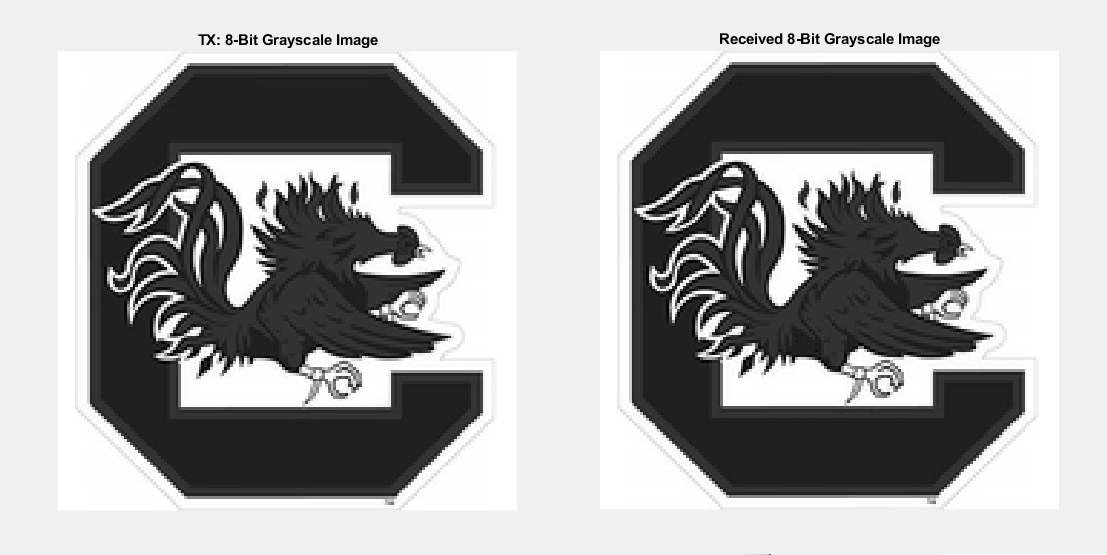
\includegraphics[scale=0.6]{8BW_image.png}
\end{center}
\begin{center}
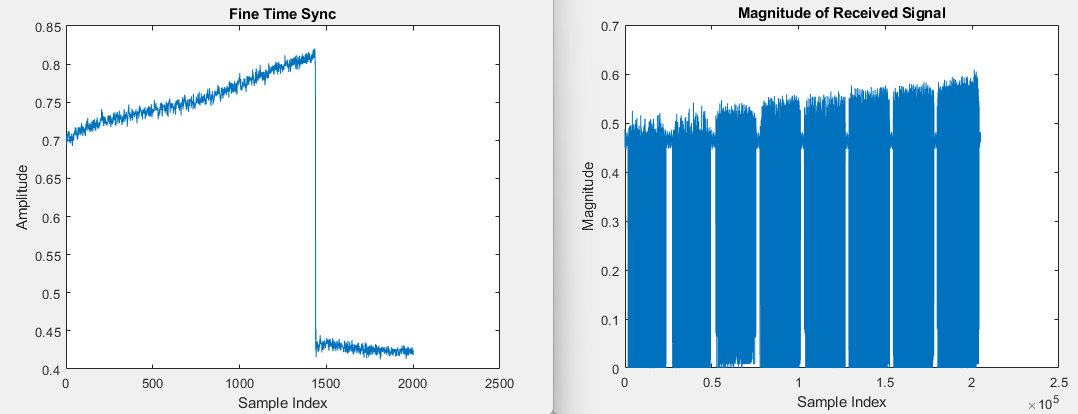
\includegraphics[scale=0.5]{8BW_Sync.png}
\end{center}
\begin{center}
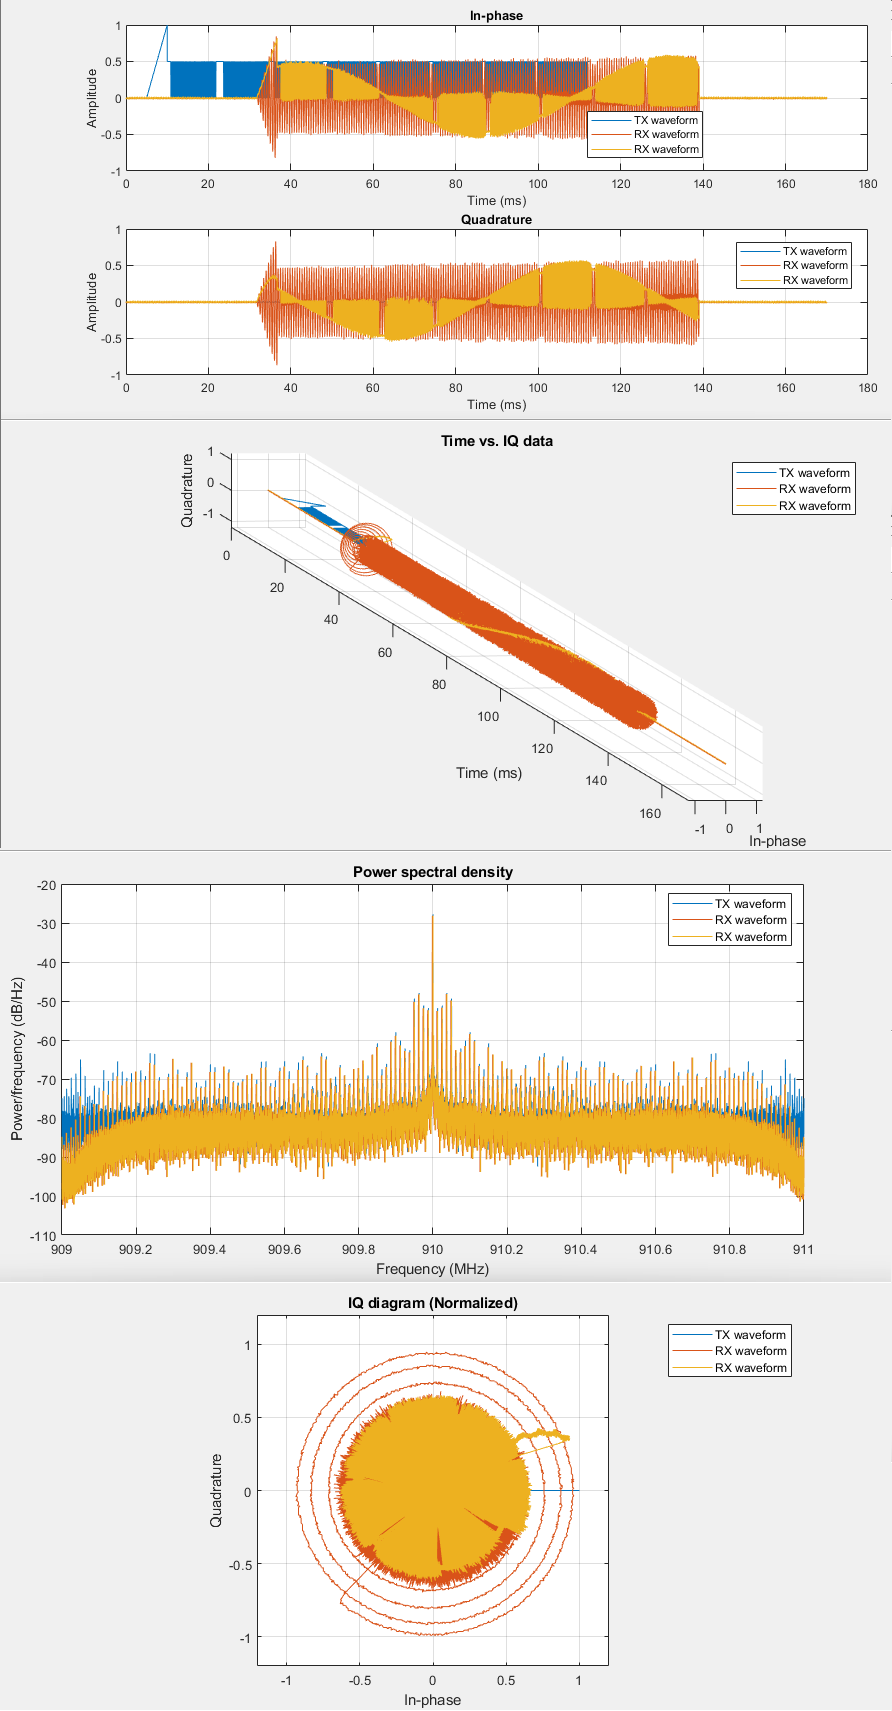
\includegraphics[scale=0.42]{8BW_results.png}
\end{center}


\end{document}
